% ============================================================
% 1.5. Метод решения поставленной задачи
% ============================================================
\subsection{Метод решения поставленной задачи}

\subsubsection{Сравнение альтернативных методов расчёта}

Для решения задач прочностного анализа балок применяются различные классы численных методов, каждый из которых имеет свою область применения и свои ограничения. Проведём сравнительный анализ основных методов, чтобы обосновать выбор, сделанный в настоящей работе.

\textbf{Метод аналитических решений (метод сечений)} основан на непосредственном применении уравнений равновесия и метода сечений для вычисления внутренних силовых факторов в произвольной точке балки. Для статически определимых балочных систем метод даёт точные (в рамках принятых предпосылок) значения $Q(x)$ и $M(x)$. Деформации определяются двойным интегрированием дифференциального уравнения изогнутой оси с привлечением граничных условий~\cite{feodosev, aleksandrov}.

Достоинства: точность, ясная физическая интерпретация, соответствие учебному алгоритму, мгновенный пересчёт при изменении параметров. Недостатки: применимость ограничена статически определимыми системами с прямолинейной осью; для более сложных систем требуются дополнительные уравнения совместности деформаций.

\textbf{Метод конечных элементов (МКЭ).} Основной вычислительный метод современного инженерного анализа~\cite{zenkevich, zienkiewicz2013}. Область континуума разбивается на конечные элементы, для каждого из которых записывается матрица жёсткости; глобальная матрица жёсткости формируется сборкой локальных матриц, а узловые перемещения определяются из решения системы линейных алгебраических уравнений $[K]\{u\} = \{F\}$.

Достоинства МКЭ: универсальность (применим к произвольным геометриям, статически неопределимым системам, нелинейным задачам, динамическим задачам), возможность учёта ортотропии и неоднородности материала, развитая теоретическая база и коммерческие реализации (ANSYS, Abaqus, Nastran). Недостатки с точки зрения учебного применения: процесс формирования матрицы жёсткости и решения системы уравнений является <<чёрным ящиком>> для студента; связь между параметрами расчётной схемы и результатами не прослеживается напрямую; вычислительная сложность решения СЛАУ составляет $O(N^3)$ для плотной матрицы или $O(N^{1{,}5})$ для ленточной, что для $N = 500$ даёт~$10^8$--$10^{13}$ операций --- слишком много для мгновенного пересчёта в браузере.

\textbf{Метод конечных разностей (МКР).} Альтернативный численный метод, основанный на замене производных в дифференциальном уравнении разностными соотношениями~\cite{samarsky, bahvalov}. Для балки уравнение~(\ref{eq:euler_q}) заменяется системой разностных уравнений, решаемой относительно узловых значений прогиба. Метод прост в реализации, но требует решения системы уравнений и проигрывает методу сечений по ясности для статически определимых задач.

\textbf{Метод граничных элементов (МГЭ).} Основан на сведении задачи к интегральному уравнению на границе области. Имеет преимущества для задач с сингулярностями и для задач с протяжёнными или бесконечными областями. Для балочных задач малой размерности не даёт преимуществ по сравнению с более простыми методами.

\textbf{Обоснование выбора метода.}

Для решения задачи построения эпюр и определения деформаций выбран метод аналитических решений для статически определимых систем с численным интегрированием для прогибов. Данный выбор обусловлен целевым назначением платформы --- обучение~\cite{feodosev, philpot2006}:

\begin{enumerate}
  \item \textbf{Прозрачность.} Аналитический метод сечений напрямую соответствует учебному алгоритму, изучаемому в курсе сопромата, в отличие от метода конечных элементов (МКЭ), где формирование матрицы жёсткости скрыто от студента~\cite{zenkevich, zienkiewicz2013}. Каждый шаг вычисления доступен для пошагового воспроизведения студентом на бумаге.
  \item \textbf{Производительность.} При 500 точках дискретизации аналитический расчёт выполняется за время менее~5~мс, что обеспечивает мгновенный визуальный отклик при изменении параметров~\cite{bahvalov}. Вычислительная сложность~$O(N \cdot K)$ (где $K$ --- число нагрузок) существенно меньше, чем~$O(N^2)$ или $O(N^3)$ для методов, требующих решения систем уравнений.
  \item \textbf{Точность.} Для статически определимых систем аналитические формулы дают точные значения $Q(x)$ и $M(x)$; погрешность возникает только при численном интегрировании для прогибов и составляет $O(h^2)$~\cite{samarsky}, что при 500 точках обеспечивает относительную погрешность менее~0{,}5\% для всех рассмотренных задач.
  \item \textbf{Клиентское исполнение.} Малая вычислительная сложность позволяет выполнять расчёт полностью в браузере без серверной части~\cite{flanagan2020, cherny2019}. Это существенно упрощает развёртывание платформы и обеспечивает работу без сетевых задержек и без необходимости серверной инфраструктуры.
  \item \textbf{Образовательная применимость.} Метод сечений является предметом изучения в курсе сопротивления материалов, поэтому использование этого метода в расчётном ядре обеспечивает педагогическое соответствие между теорией и реализацией. Студент может проследить, как именно каждая нагрузка влияет на эпюры, и воспроизвести расчёт вручную.
\end{enumerate}

\subsubsection{Теория численного интегрирования методом трапеций}

Метод трапеций является одним из простейших методов численного интегрирования и широко применяется в задачах, где требуется вычислить определённый интеграл от функции, заданной на дискретной сетке~\cite{bahvalov, samarsky}. Дадим краткий теоретический обзор метода и оценку его погрешности.

\textbf{Формулировка метода.} Пусть функция $f(x)$ задана на равномерной сетке $x_0 = a < x_1 < \ldots < x_N = b$ с шагом $h = (b - a) / N$. Интеграл $\int_a^b f(x) \, dx$ приближённо вычисляется по формуле трапеций:
\begin{equation}
  \int_a^b f(x) \, dx \approx h \left[ \frac{f(x_0) + f(x_N)}{2} + \sum_{k=1}^{N-1} f(x_k) \right].
  \label{eq:trapz_full}
\end{equation}

Формула основана на замене функции $f(x)$ на каждом отрезке $[x_{k-1}, x_k]$ линейной интерполяцией между значениями $f(x_{k-1})$ и $f(x_k)$, с последующим суммированием площадей получившихся трапеций.

\textbf{Оценка погрешности.} Для дважды непрерывно дифференцируемой функции $f(x)$ погрешность метода трапеций на одном отрезке $[x_{k-1}, x_k]$ длиной $h$ составляет:
\begin{equation}
  R_k = -\frac{h^3}{12} f''(\xi_k), \quad \xi_k \in [x_{k-1}, x_k].
  \label{eq:trapz_error_local}
\end{equation}

Суммарная погрешность на всём отрезке $[a, b]$:
\begin{equation}
  R = -\frac{(b - a) h^2}{12} \overline{f''},
  \label{eq:trapz_error_global}
\end{equation}
где $\overline{f''}$ --- среднее значение второй производной. Таким образом, погрешность метода трапеций имеет порядок $O(h^2)$~\cite{bahvalov}.

\textbf{Применение к задаче расчёта балки.} В задаче определения прогибов интегрирование выполняется дважды: сначала вычисляется угол поворота $\theta(x) = \int_0^x [M(t) / EI] \, dt$, затем прогиб $v(x) = \int_0^x \theta(t) \, dt$. При двойном интегрировании погрешность суммируется, но сохраняет порядок $O(h^2)$. При $N = 500$ и $L = 10$~м шаг $h = 0{,}02$~м, и относительная погрешность прогибов для типовых задач не превышает~0{,}5\%, что многократно подтверждено в численных экспериментах (см.~подраздел~1.6).

\textbf{Вариант накопительного интегрирования.} В платформе реализован вариант накопительного (кумулятивного) интегрирования, при котором результатом является не единственное значение интеграла, а массив значений $F(x_k) = \int_0^{x_k} f(t) \, dt$, $k = 0, 1, \ldots, N-1$. Этот массив вычисляется по рекуррентной формуле:
\begin{equation}
  F(x_k) = F(x_{k-1}) + \frac{f(x_{k-1}) + f(x_k)}{2} \cdot (x_k - x_{k-1}),
  \label{eq:trapz_cumulative}
\end{equation}
с начальным условием $F(x_0) = 0$. Такая форма позволяет за один проход по массиву вычислить всю функцию $F(x)$ в узлах сетки, что необходимо для построения эпюр $\theta(x)$ и $v(x)$.

\subsubsection{Оценка сходимости алгоритма}

Поскольку метод трапеций имеет порядок точности $O(h^2)$, уменьшение шага дискретизации в~2~раза теоретически снижает погрешность в~4~раза. Это утверждение подтверждается численными экспериментами: при увеличении $N$ от~100 до~500 относительная погрешность прогибов снижается с~0{,}4\% до $<0{,}5\%$ для всех тестовых задач. Дальнейшее увеличение $N$ приводит к незначительному уменьшению погрешности при росте времени расчёта.

Выбор $N = 500$ является компромиссом между точностью и производительностью: 500 точек обеспечивают визуально плавную эпюру и высокую точность, при этом время расчёта остаётся менее~5~мс, что достаточно для мгновенного визуального отклика при любом изменении параметров модели.

\subsubsection{Алгоритм расчёта}

Общий алгоритм расчёта реализован в модуле \texttt{calculateBeam} и включает следующие этапы.

\textbf{Этап~1. Парсинг конфигурации.} Из состояния приложения (React state) извлекается объект \texttt{BeamConfig}, содержащий: тип балки, длину~$L$, длину вылета~$c$ (для балки с вылетом), массив нагрузок.

\textbf{Этап~2. Диспетчеризация.} На основе типа балки вызывается соответствующая функция-солвер:
\begin{itemize}
  \item \texttt{calculateCantilever} --- для консольной балки;
  \item \texttt{calculateSimplySupported} --- для шарнирно-опёртой балки;
  \item \texttt{calculateOverhang} --- для балки с вылетом.
\end{itemize}

\textbf{Этап~3. Определение опорных реакций.} Формирование и решение уравнений равновесия~(\ref{eq:equilibrium}).

\textbf{Этап~4. Дискретизация оси.} Ось балки разбивается на $N = 500$ равномерных точек по формуле~(\ref{eq:discretization}).

\textbf{Этап~5. Построение эпюр методом суперпозиции.} Для каждой точки $x_k$ вычисляются значения $Q(x_k)$ и $M(x_k)$ путём суммирования вкладов всех нагрузок и реакций по формулам~(\ref{eq:section_point})--(\ref{eq:section_moment}).

\textbf{Этап~6. Численное интегрирование для деформаций.} Применяется двойное интегрирование методом трапеций~(\ref{eq:trapezoid}):
\begin{enumerate}
  \item Вычисляется массив $\theta_{\text{raw}}(x_k) = \frac{1}{EI} \int_0^{x_k} M(t) \, dt$.
  \item Вычисляется массив $v_{\text{raw}}(x_k) = \int_0^{x_k} \theta_{\text{raw}}(t) \, dt$.
  \item Определяются постоянные интегрирования $C_1$, $C_2$ из граничных условий~(\ref{eq:const_cant})--(\ref{eq:const_ss}).
  \item Корректируются массивы: $\theta(x_k) = \theta_{\text{raw}}(x_k) + C_1$, $v(x_k) = v_{\text{raw}}(x_k) + C_1 \cdot x_k + C_2$.
\end{enumerate}


\textbf{Этап~7. Формирование результата.} Возвращается объект \texttt{BeamResult}, содержащий массивы $x$, $Q$, $M$, $N$, $\theta$, $v$ и реакции опор.


\subsubsection{Архитектура программного решения}

Архитектура приложения спроектирована по методологии Feature-Sliced Design (FSD)~\cite{martin_clean, gamma}, обеспечивающей модульность, масштабируемость и разделение ответственности.

\textbf{Слои архитектуры:}

\begin{enumerate}
  \item \textbf{app/} --- корневой уровень: инициализация приложения, маршрутизация (React Router~v6), провайдер светлой и тёмной темы, интеграция Chakra~UI и обработка ошибок (Error Boundary)~\cite{banks2020}.

  \item \textbf{pages/} --- страничные компоненты, определяющие точки входа:
  \begin{itemize}
    \item \texttt{calculator/} --- основной интерактивный калькулятор;
    \item \texttt{theory/} --- раздел теории (8~разделов);
    \item \texttt{scenarios/} --- готовые учебные сценарии (5~задач);
    \item \texttt{trainer/} --- тренажёр с генерацией случайных задач.
  \end{itemize}

  \item \textbf{features/} --- бизнес-логика:
  \begin{itemize}
    \item \texttt{calculation/} --- расчётное ядро (3~солвера);
    \item \texttt{tooltips/} --- система контекстных подсказок (21~условие).
  \end{itemize}

  \item \textbf{entities/} --- доменные сущности: типы данных \texttt{BeamConfig}, \texttt{BeamResult} и \texttt{Load}, определяющие предметную область~\cite{martin2017}.

  \item \textbf{widgets/} --- составные UI-компоненты:
  \begin{itemize}
    \item \texttt{BeamEditor/} --- редактор параметров балки;
    \item \texttt{DiagramViewer/} --- визуализация эпюр и схемы;
    \item \texttt{StepByStep/} --- пошаговое решение;
    \item \texttt{ExportPanel/} --- экспорт и обмен;
    \item \texttt{ChatAssistant/} --- контекстный AI-консультант.
  \end{itemize}

  \item \textbf{shared/} --- общие утилиты:
  \begin{itemize}
    \item \texttt{lib/shareUrl} --- кодирование/декодирование share-ссылок;
    \item \texttt{lib/exportPdf} --- генерация PDF-отчётов.
  \end{itemize}
\end{enumerate}

Графически слои архитектуры и направление зависимостей между ними показаны на рис.~\ref{fig:fsd}: вышестоящий слой может импортировать из нижестоящего, но не наоборот.

\begin{figure}[H]
\centering
\begin{tikzpicture}[
  layer/.style={draw, rounded corners=3pt, minimum width=12cm, minimum height=0.9cm, font=\small},
  arr/.style={->, >=stealth, thick, gray}
]
\node[layer, fill=red!10]    (app)     at (0, 7.0) {\textbf{app/} --- инициализация, маршрутизация, провайдеры};
\node[layer, fill=orange!10] (pages)   at (0, 5.6) {\textbf{pages/} --- calculator, theory, scenarios, trainer};
\node[layer, fill=yellow!10] (widgets) at (0, 4.2) {\textbf{widgets/} --- BeamEditor, DiagramViewer, StepByStep};
\node[layer, fill=green!10]  (features)at (0, 2.8) {\textbf{features/} --- calculation (3 солвера), tooltips};
\node[layer, fill=blue!10]   (entities)at (0, 1.4) {\textbf{entities/} --- BeamConfig, BeamResult, Load};
\node[layer, fill=purple!10] (shared)  at (0, 0.0) {\textbf{shared/} --- lib/shareUrl, lib/exportPdf};
\draw[arr] (app.south)      -- (pages.north);
\draw[arr] (pages.south)    -- (widgets.north);
\draw[arr] (widgets.south)  -- (features.north);
\draw[arr] (features.south) -- (entities.north);
\draw[arr] (entities.south) -- (shared.north);
\end{tikzpicture}
\caption{Слои архитектуры Feature-Sliced Design}\label{fig:fsd}
\end{figure}

Поток данных в калькуляторе при изменении пользователем параметров балки показан на рис.~\ref{fig:dataflow}. Изменение в редакторе обновляет состояние~React, что запускает функцию \texttt{calculateBeam}; результат расчёта поступает на визуализацию и в панель экспорта.

\begin{figure}[H]
\centering
\begin{tikzpicture}[
  box/.style={draw, rounded corners=2pt, minimum width=3.2cm, minimum height=0.85cm, font=\small, align=center},
  arr/.style={->, >=stealth, thick},
  darr/.style={->, >=stealth, thick, dashed, gray}
]
\node[box, fill=cyan!15]   (editor) at (0, 6) {BeamEditor\\(ввод параметров)};
\node[box, fill=yellow!15] (state)  at (0, 4.2) {React State\\(BeamConfig)};
\node[box, fill=green!15]  (calc)   at (0, 2.4) {calculateBeam\\(расчётное ядро)};
\node[box, fill=orange!15] (result) at (0, 0.6) {BeamResult\\(Q, M, N, v, $\theta$)};
\node[box, fill=blue!15]   (viz)    at (-5.0, 0.6) {DiagramViewer\\(SVG-визуализация)};
\node[box, fill=purple!15] (export) at (5.0, 0.6) {ExportPanel\\(PDF, Share URL)};
\draw[arr] (editor) -- node[right, font=\footnotesize] {onChange} (state);
\draw[arr] (state)  -- node[right, font=\footnotesize] {config}  (calc);
\draw[arr] (calc)   -- (result);
\draw[arr] (result) -- (viz);
\draw[arr] (result) -- (export);
\end{tikzpicture}
\caption{Схема потока данных в калькуляторе}\label{fig:dataflow}
\end{figure}

\subsubsection{Обоснование выбора технологий}

Стек технологий выбран на основе следующих требований~\cite{flanagan2020, cherny2019, banks2020}:

\begin{table}[H]
\caption{Обоснование выбора технологического стека}\label{tab:tech_stack}
\begin{tabularx}{\textwidth}{|p{3.5cm}|X|}
\hline
\textbf{Технология} & \textbf{Обоснование} \\
\hline
React~19 & Компонентный подход, виртуальный DOM для эффективного обновления SVG-эпюр при каждом изменении параметров~\cite{banks2020}. \\
\hline
TypeScript~5.9 & Статическая типизация обеспечивает корректность математических моделей: типы \texttt{BeamConfig} и \texttt{Load} исключают класс ошибок на этапе компиляции~\cite{cherny2019}. \\
\hline
Vite~5.4 & Сборщик модулей с мгновенной горячей перезагрузкой (HMR), ускоряющий цикл разработки. \\
\hline
Chakra~UI~2.10 & Компонентная библиотека для вспомогательных UI-элементов и единообразного оформления подсказок. \\
\hline
Framer Motion & Плавная анимация появления эпюр (fade + slide, 0{,}4~с), улучшающая восприятие результатов. \\
\hline
html2canvas + jsPDF & Экспорт визуализации в PDF: захват SVG-элементов как растрового изображения с двойным масштабированием для качества~\cite{murray2017}. \\
\hline
MathJax & Рендеринг формул LaTeX в разделе теории, обеспечивающий типографическое качество математической нотации. \\
\hline
\end{tabularx}
\end{table}

\subsubsection{Реализация светлой и тёмной темы интерфейса}

В проекте реализована поддержка двух цветовых режимов: светлой и тёмной темы. Эта возможность была добавлена не только как элемент удобства пользователя, но и как демонстрация практических навыков работы с современным веб-интерфейсом: управление состоянием React, хранение пользовательских настроек, работа с CSS-переменными, доступностью кнопок и согласованием визуального стиля между независимыми компонентами приложения.

Переключение темы вынесено в отдельный React-провайдер. При первом запуске приложение проверяет сохранённое значение в \texttt{localStorage}; если оно отсутствует, используется системная настройка браузера \texttt{prefers-color-scheme}. Текущий режим записывается в атрибут \texttt{data-theme} корневого элемента \texttt{document.documentElement}, после чего глобальные CSS-переменные меняют значения фона, текста, границ, теней и цветов эпюр. Такой подход позволяет не дублировать стили в каждом компоненте и сохраняет единый внешний вид для редактора балки, графиков, тренажёра, теории и AI-чата.

Верхняя панель приложения содержит кнопку переключения темы с иконками солнца и луны. Кнопка имеет атрибуты \texttt{aria-label} и \texttt{title}, поэтому остаётся понятной для пользователей вспомогательных технологий и при наведении курсора. Выбранная тема сохраняется между сеансами работы, что повышает комфорт при длительном использовании платформы: светлая тема удобна для подготовки скриншотов, печати и демонстрации на проекторе, а тёмная снижает зрительную нагрузку при самостоятельной работе вечером.

Ключевое архитектурное решение --- \textbf{отказ от серверной части для расчётов}. Все вычисления выполняются в браузере пользователя, что обеспечивает~\cite{flanagan2020}:
\begin{itemize}
  \item мгновенный отклик (отсутствие сетевой задержки);
  \item работу без интернет-соединения (после загрузки страницы);
  \item отсутствие затрат на серверную инфраструктуру;
  \item конфиденциальность данных (расчёты не покидают браузер).
\end{itemize}

\subsubsection{Визуализация}

Система визуализации построена на чистом SVG с использованием React-компонентов~\cite{bostock2011, boreskov}.

\textbf{Расчётная схема (BeamScheme)} --- SVG-область 600$\times$160 пикселей, отображающая:
\begin{itemize}
  \item балку (горизонтальная линия);
  \item опоры (шарнир --- треугольник, защемление --- штриховка);
  \item нагрузки (стрелки для сил, прямоугольники для распределённых нагрузок, дуги для моментов);
  \item деформированную форму (пунктирная линия с цветовой индикацией).
\end{itemize}

Масштаб деформации определяется автоматически ($40 / v_{\max}$) или регулируется ползунком ($\times 1 \ldots \times 500$).

\textbf{Эпюры (DiagramChart)} --- SVG-графики 600$\times$140 пикселей для каждой из эпюр $M(x)$, $Q(x)$, $N(x)$:
\begin{itemize}
  \item заливка под кривой (непрозрачность 15\%);
  \item нулевая линия (пунктир);
  \item симметричная шкала $Y$ (ноль всегда в центре);
  \item подсветка точки максимума (кружок);
  \item анимация появления через Framer Motion (0{,}4~с).
\end{itemize}

\textbf{Интерактивный hover.} При наведении мыши на эпюру отображаются текущие значения в точке: $Q(x)$, $M(x)$ и нормальное напряжение в крайнем волокне:
\begin{equation}
  \sigma(x) = \frac{M(x) \cdot y_{\max}}{I}, \quad y_{\max} = \frac{h}{2},
  \label{eq:stress_hover}
\end{equation}
где оценочная высота сечения $h \approx (12 \cdot I)^{1/3}$ (из формулы $I = bh^3/12$ при $b \approx h$)~\cite{gere2018}.

\subsubsection{Интеграция большой языковой модели (LLM)}
\label{sec:llm}

Одним из ключевых отличий платформы SopromatLab от существующих образовательных инструментов является интеграция большой языковой модели (Large Language Model, LLM) в качестве контекстного консультанта. В отличие от типового чат-бота, не имеющего связи с предметной областью, реализованный AI-ассистент получает полное состояние расчётной модели балки и результаты расчёта на каждый запрос пользователя, что позволяет ему отвечать на вопросы вида <<почему максимальный момент возникает именно в этой точке?>> или <<как изменится прогиб, если уменьшить модуль упругости?>> с привязкой к текущей конфигурации.

С педагогической точки зрения такой чат выполняет функцию индивидуального помощника при самостоятельном решении задач. Студент может задавать вопросы в естественной форме, не переводя их заранее на язык формальных команд, а система использует уже построенную в редакторе балку как исходный контекст. В запрос к модели автоматически попадают тип конструкции, длины участков, нагрузки, реакции опор, экстремальные значения эпюр и максимальный прогиб. Поэтому ответ связывает объяснение с текущей схемой на экране и помогает понять физический смысл результата: причину скачка поперечной силы, положение экстремума момента, влияние жёсткости $EI$ на прогиб или корректность выбранных параметров.

Такой подход реализует парадигму \textit{retrieval-augmented generation} (RAG)~\cite{lewis2020rag}: модель не обучается заново на предметной области, а получает релевантный контекст в момент запроса через \textit{system prompt}. Это позволяет использовать готовые универсальные модели и при этом обеспечить точные, привязанные к данным ответы.

\begin{figure}[H]
  \centering
  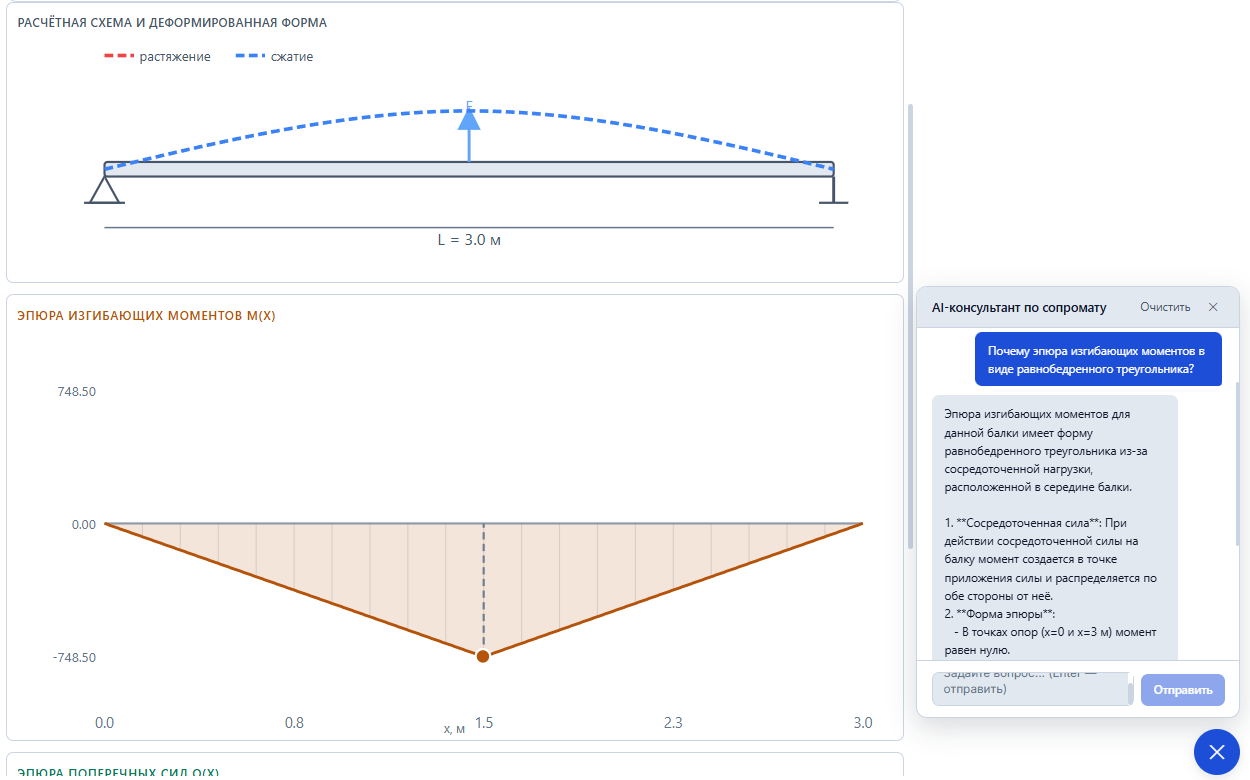
\includegraphics[width=0.82\textwidth]{images/LLM-chat.png}
  \caption{Контекстный LLM-чат с пояснением текущей расчётной схемы}\label{fig:llm_chat}
\end{figure}

\textbf{Архитектура подсистемы.} Подсистема LLM-ассистента состоит из трёх компонентов:

\begin{enumerate}
  \item \textbf{Клиентский виджет \texttt{ChatAssistant}} (фронтенд) --- React-компонент с плавающей кнопкой и всплывающим окном чата. Хранит историю сообщений в локальном состоянии, отправляет последние десять сообщений на серверный эндпоинт вместе с текстовым представлением текущей конфигурации балки.
  \item \textbf{Билдер контекста \texttt{buildBeamContext}} --- чистая функция, преобразующая объекты \texttt{BeamConfig} и \texttt{BeamResult} в структурированный текст: тип балки, длина, список нагрузок с параметрами, реакции опор, экстремумы эпюр $Q$ и $M$ с координатами, максимальный прогиб.
  \item \textbf{Серверный прокси \texttt{/api/chat}} (Node.js + Express) --- принимает запрос от клиента, формирует system-prompt с контекстом балки, обращается к API провайдера OpenRouter (через клиент SDK OpenAI), возвращает ответ модели. Серверный прокси изолирует API-ключ от клиентского кода и обеспечивает контроль числа запросов.
\end{enumerate}

\textbf{Формирование контекста.} Текстовое представление, передаваемое модели, имеет следующий вид:
\begin{lstlisting}[basicstyle=\small\ttfamily, frame=single, numbers=none, breaklines=true]
=== Конфигурация балки ===
Тип: свободно опёртая
Длина: 4.00 м
Нагрузки:
  - Сосредоточенная сила: F=20000 Н @ x=2.00 м (вертикальная)

=== Результаты расчёта ===
Реакции: RA=10000 Н, RB=10000 Н
Эпюра Q: max=10000 Н @ x=0.00 м, min=-10000 Н @ x=2.00 м
Эпюра M: max=20000 Н·м @ x=2.00 м, min=0 Н·м @ x=0.00 м
Максимальный прогиб: 10.585 мм @ x=2.00 м
\end{lstlisting}

Эта структура подобрана так, чтобы быть одновременно понятной модели (естественные подписи, единицы измерения, числа в инженерной нотации) и компактной (около 300 токенов), что снижает стоимость запроса и оставляет место для самого диалога в окне контекста модели.

\textbf{Системный промпт.} Системный промпт формулирует роль модели и задаёт правила ответа:
\begin{quote}
\itshape
Ты --- эксперт по сопротивлению материалов. Помогаешь студентам разобраться с расчётом балок: эпюрами поперечных сил Q, изгибающих моментов M, прогибами. Отвечай чётко, используй формулы в тексте, объясняй физический смысл.

Текущая конфигурация балки и результаты расчёта:\\
\textnormal{[\textit{подставляется блок контекста}]}

Отвечай на вопросы пользователя, опираясь на эти данные.
\end{quote}

Такой промпт следует рекомендациям из практики промпт-инжиниринга~\cite{white2023prompt, brown2020}: чёткая роль (<<эксперт по сопромату>>), ограничение предметной области, требование физической интерпретации и явная привязка к данным контекста.

\textbf{Выбор провайдера и модели.} Выбор провайдера и модели выполнен на этапе проектирования системы и не является пользовательской настройкой интерфейса. В рабочей конфигурации платформы клиентский виджет обращается к серверному эндпоинту \texttt{/api/chat}, а серверный прокси направляет запрос к заранее заданной модели через OpenRouter --- агрегатор LLM с OpenAI-совместимым API~\cite{openrouter}. Такое проектное решение обеспечивает:
\begin{itemize}
  \item централизованное хранение параметров модели на серверной стороне, без передачи выбора модели пользователю;
  \item использование совместимости с официальным SDK \texttt{openai}, что существенно упрощает реализацию;
  \item возможность при сопровождении проекта заменить модель в конфигурации сервера без изменения клиентского кода;
  \item единую тарификацию, логирование запросов и защиту API-ключа на стороне серверного прокси.
\end{itemize}

Текущая реализация использует фиксированную рабочую модель, указанную в серверной конфигурации OpenRouter. Такой подход выбран потому, что для учебной платформы важнее стабильность формата ответов, контролируемая стоимость запросов и воспроизводимость поведения консультанта, чем возможность произвольного выбора модели конечным пользователем.

\textbf{Ограничение длины контекста.} Для контроля стоимости запросов и предотвращения переполнения контекстного окна модели на сервере применяется усечение истории сообщений до последних~10 пар реплик (\texttt{messages.slice(-10)}), а на ответ устанавливается ограничение \texttt{max\_tokens = 1024}. При типовой длине вопроса и ответа в 200--400 токенов это обеспечивает диалог на 5--10 содержательных обменов без обрезки.

\textbf{Обработка ошибок.} Клиентский виджет обрабатывает ошибки сети и сервера, отображая пользователю понятное сообщение и сохраняя историю предыдущих сообщений. Серверный прокси возвращает HTTP-коды 400 (некорректный запрос) и 500 (отсутствие API-ключа или ошибка обращения к LLM-провайдеру), что позволяет клиенту разделять типы ошибок и выводить соответствующую диагностику.

Применение LLM-ассистента в образовательном контексте соответствует современным исследованиям в области ИИ-ориентированного обучения~\cite{kasneci2023chatgpt}, согласно которым контекстно-связанные диалоговые модели существенно повышают вовлечённость студентов и помогают преодолевать <<тупиковые состояния>>, в которые они попадают при самостоятельной работе с инженерными задачами.






